\documentclass[journal]{IEEEtran}

\hyphenation{op-tical net-works semi-conduc-tor}

\usepackage{amsmath}
\usepackage{amssymb}
\usepackage{amsthm}
\usepackage{graphicx}
\usepackage{hyperref}

\newtheorem{mydef}{Definition}
\newtheorem{mylem}{Lemma}
\newtheorem{mythm}{Theorem}
\newtheorem{myprop}{Property}
\newtheorem{mycoro}{Corollary}


\begin{document}

\title{Input-to-state stable analysis on Particle Swarm Optimization}

\author{
\IEEEauthorblockN{Daqing Yi,
Kevin D. Seppi, and Michael A. Goodrich}

\IEEEauthorblockA{Department of computer science, Brigham Young University, Provo, UT 84604 USA}
\thanks{}
}

% The paper headers
%\markboth{Journal of \LaTeX\ Class Files,~Vol.~11, No.~4, December~2012}%
%{Shell \MakeLowercase{\textit{et al.}}: Bare Demo of IEEEtran.cls for Journals}
\markboth{}{}

\maketitle

\begin{abstract}
This paper examines the dynamics of particle swarm optimization (PSO) by modeling PSO as a cascade system and then applying input-to-state stability analysis.
Using a cascade system model we can
include the effects of the global-best and personal-best values more directly in the model of the dynamics.
Thus in contrast to previous study of PSO dynamics, the input-to-state stability property used here allows for the analysis of PSO both before and at stagnation.
In addition, the use of input-to-state stability allows this analysis to preserve random terms which were heretofore simplified to constants.
This analysis is important because it can inform the setting of PSO parameters and better characterize the nature of PSO as a dynamic system.
This work also illuminates the way in which the personal best and the global best updates influence the bound on particle's position and hence, how the algorithm
exploits and explores the fitness landscape as a function of the personal best and global best.
\end{abstract}

\begin{IEEEkeywords}
Particle swarm optimization
\end{IEEEkeywords}

\IEEEpeerreviewmaketitle

\section{Introduction}

\begin{frame}{Modeling human intent}{Path Planning}
THe problem in modeling human intent
\begin{itemize}
\item incomparability in objectives
\item conflict in objectives
\item hardness in weighing the objectives
\item vagueness in importance selection
\end{itemize}
\begin{figure}
\centering
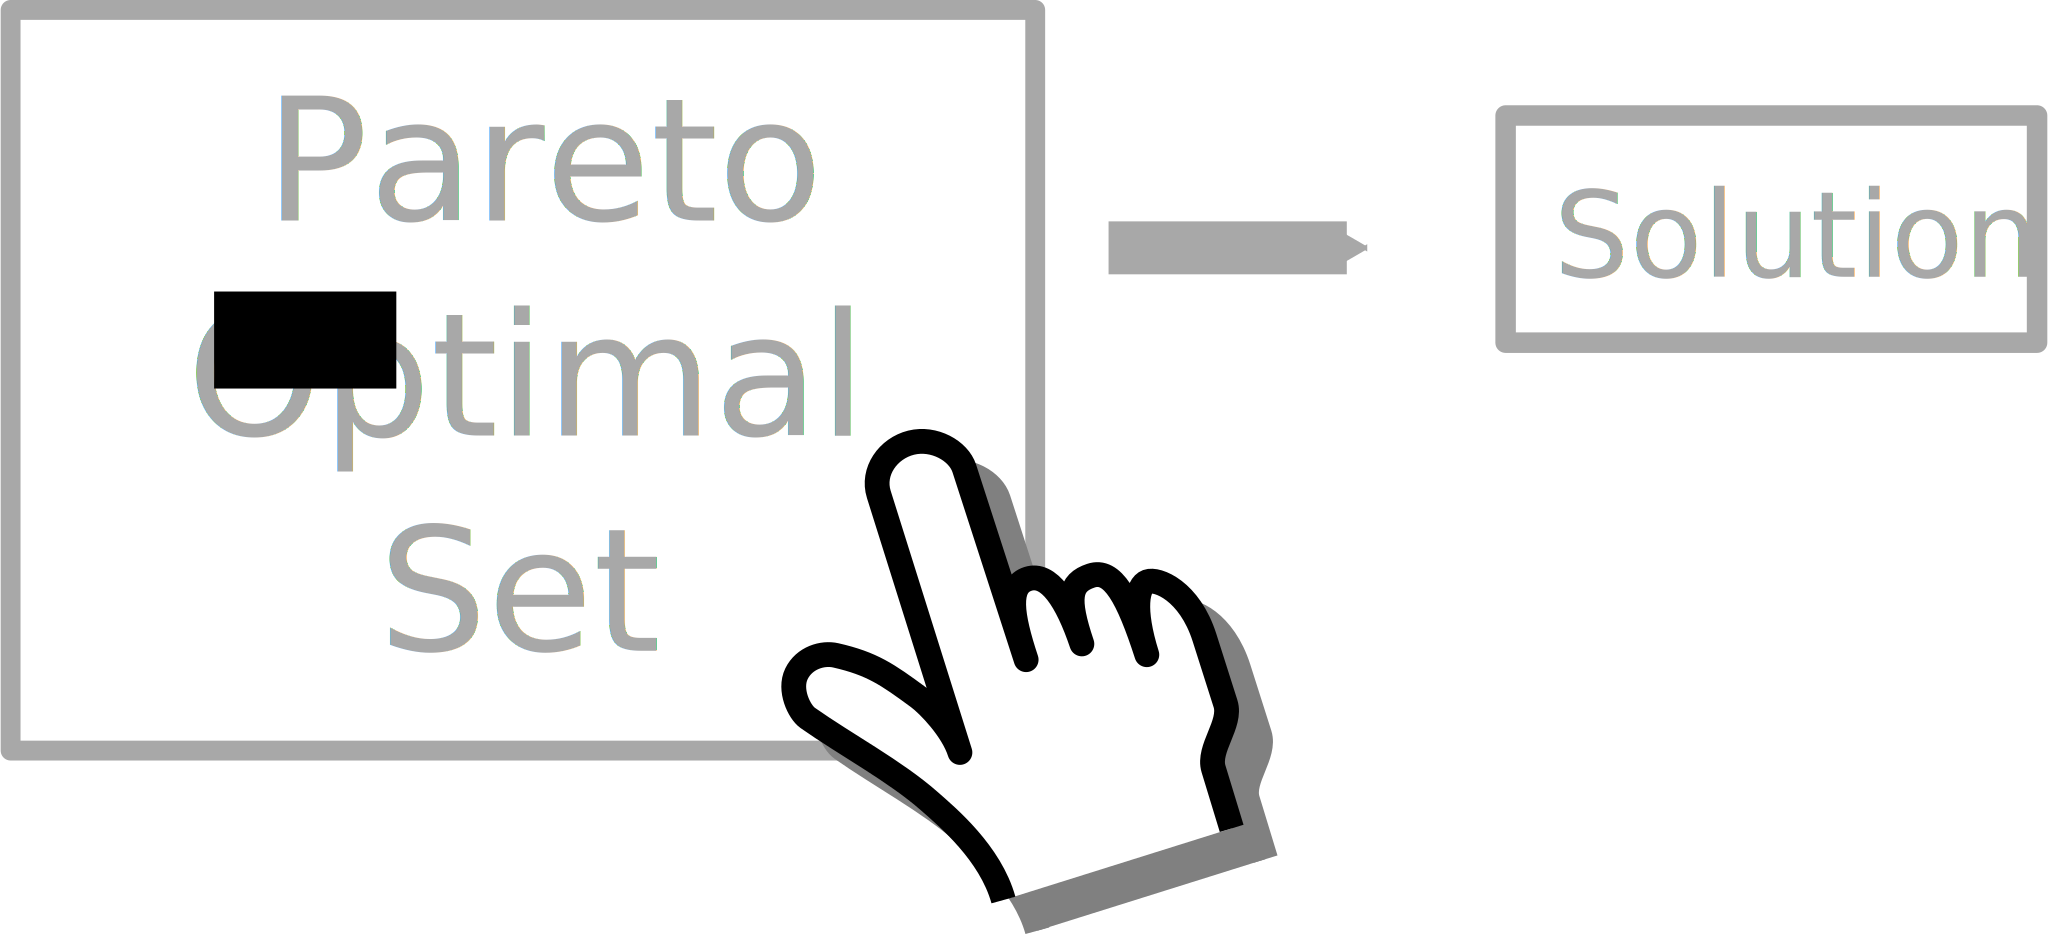
\includegraphics[width=0.6\linewidth]{figure/human_interactive_moo}
%\caption{}
\label{fig:human_interactive_moo}
\end{figure}
\end{frame}

\begin{frame}{Pareto Optimal}{}
\end{frame}

\section{Related Work}
\label{sec:related_work}

If we assume that search targets are static in the search environment, the scan on a location decreases the estimated probability that there is some search target here.
Observations in a search process reduce the uncertainty of where search targets locate.
By measuring this type of uncertainty with information, a search agent can collect more information at non-observed locations than observed ones.
Information gathering is usually selected to measure the efficiency of a search task.
In this paper, we focus on path planning in a search task answers how to maximize information with limited time and resource by defining objective in forms of information evaluation \cite{goodrich2013toward}.

Research work on information maximization path planning focuses a lot on how to solve the optimization problems defined in large scale solution spaces in reasonable time.
\cite{levine2010information} imports ideas of RRT to an information-rich path planning problem, which targets at bringing good efficiency in online optimization in a continuous space.
Under a temporal logic constraint, \cite{JonesSchwagerBeltaICRA13scLTLInfo} use a receding horizon planning to solve an online information-gathering optimization problem.

\begin{figure}
\centering
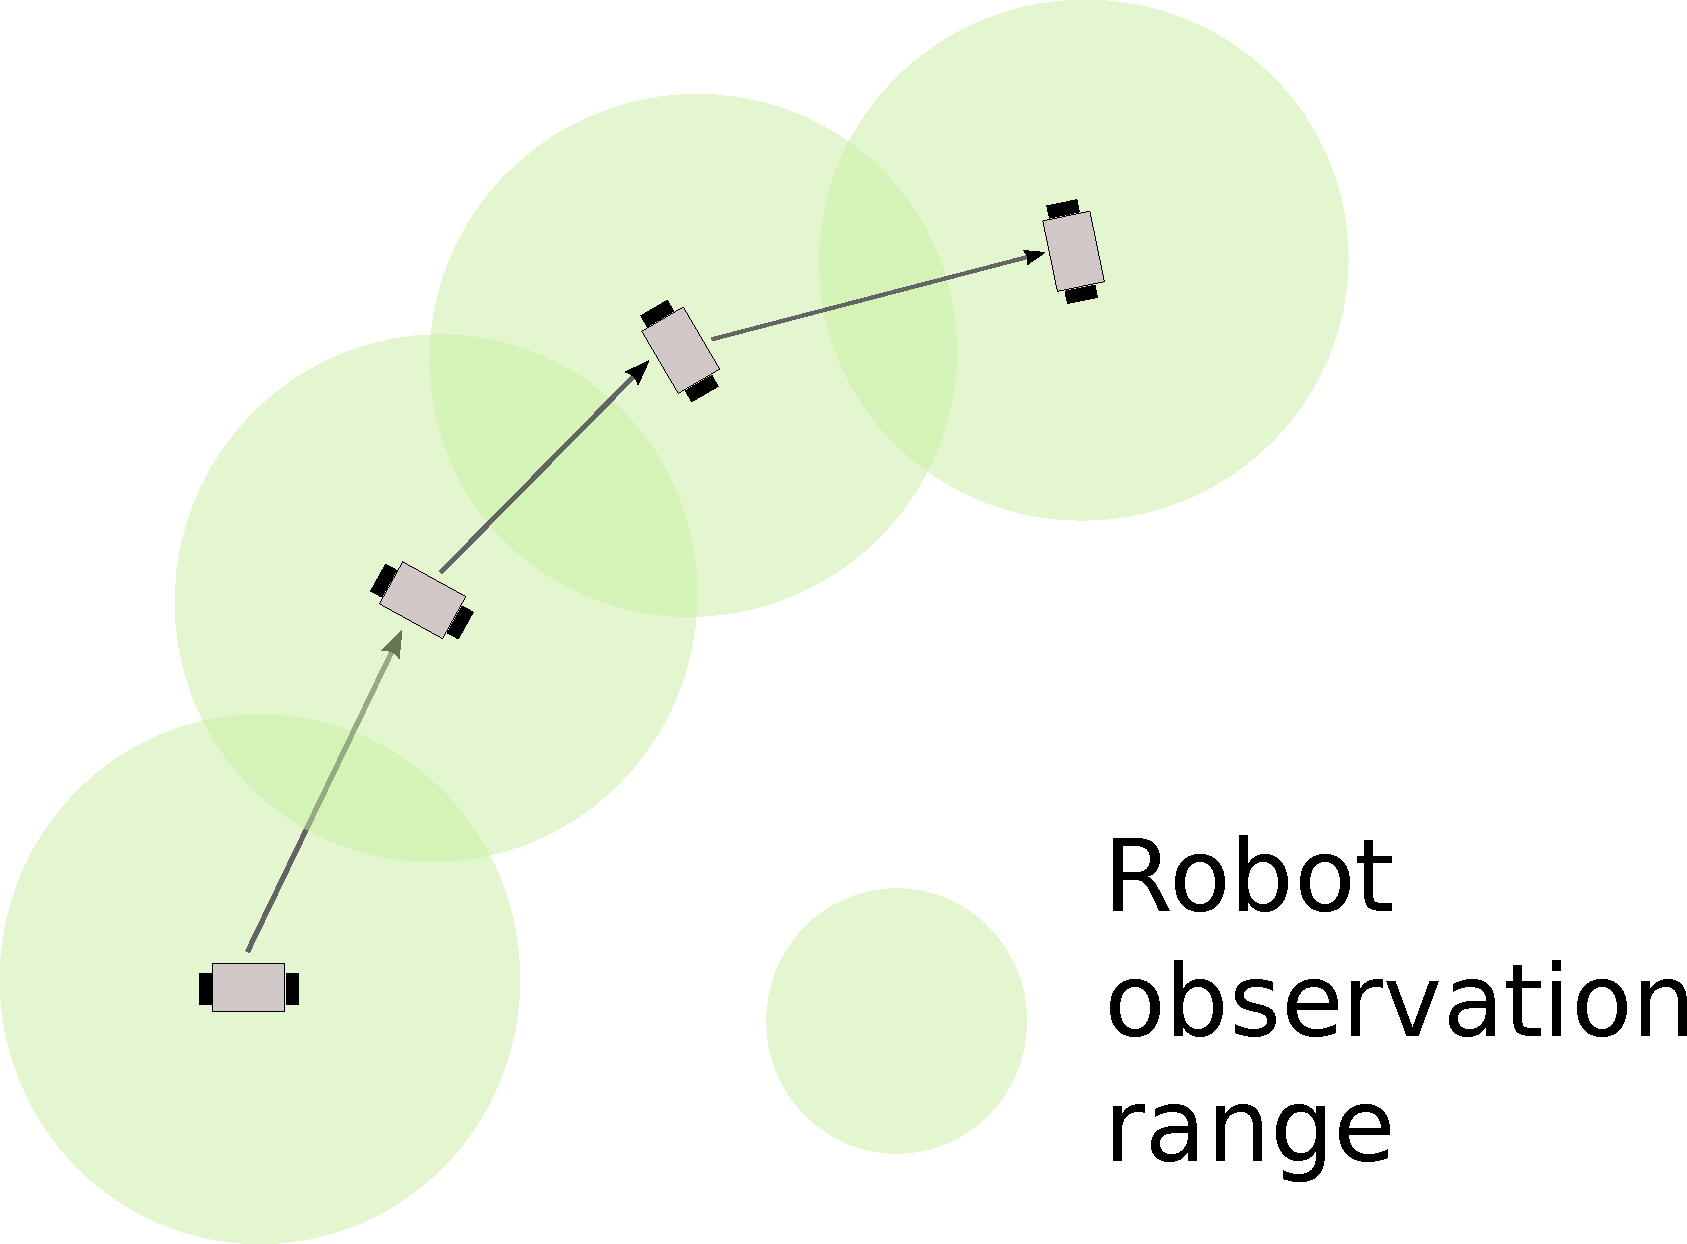
\includegraphics[width=0.4\linewidth]{./images/robotObservation.pdf}
\caption{Maximum coverage in robot observation.}
\label{fig:robotObservation}
\end{figure}

Usually the observation of a search agent covers a much larger region than the area occupied by the robot's body, which is shown in Figure \ref{fig:robotObservation}.
If we consider the observation as a covering range instead of a cell or a point, the overlaps between observation coverage at different time steps must be considered when measuring the total quantity of information.
Figure \ref{fig:robotObservation} gives an example.

Mutual information and conditional mutual information are commonly used to model the overlaps in measuring the total information \cite{singh2009efficient}.
This belongs to a \emph{maximum coverage problem}. 
Multiple sensors placement is one of the applications on information maximization.
In a sequential placement, the locations of placed sensors determine the increase on total information by adding a new sensor.
It is known to be a classical NP-hard combinatorial optimization problem \cite{megiddo1983maximum}.
The problem of maximum coverage on information measurement implies a property of ``nondecreasing submodularity''. 

Maximizing the score collected from a limited-length graph walk is usually known as an \emph{orienteering problem} \cite{Vansteenwegen20111}, in which the total score is a summation of the scores of visited vertices.
If the score function of a vertex has submodularity as in a \emph{maximum coverage problem}, the problem is defined as a \emph{submodular orienteering problem} \cite{chekuri2005recursive}.
A greedy approximation with known performance bound proposed in \cite{singh2009efficient} efficiently exploits the submodularity property of mutual information.
Similarly, in a branch and bound way, \cite{binney2012branch} apply greedy search to informative path planning.
Because the location of the robot at time $ t $ constrains the reachable location at time $ t+1 $, applying greedy algorithm with ``teleport'' assumption to the problem with this constraint can be extremely bad \cite{krause2012submodular}.
In non-teleport motion, \cite{chekuri2005recursive} import recursive greedy by converting to a knapsack constraint so that there is a time resource allocation on planning steps.

Due to the wingman constraint, the path planning of a robot wingman depends on a temporal-space synchronization requirement determined by the positions of a human through time.
The time allocation is fixed and depends on how the human's positions are sampled.
Thus we are not able to model time resource as budget in \cite{chekuri2005recursive}.   

We define the path planning of the robot wingman in a search task as an information maximization problem on a topological graph. We propose an algorithm to solve it as submodular orienteering . The algorithm is designed to produce acceptable robot performance and to be computed efficiently. We then use simulation to demonstrate the acceptable performance of the algorithm and computation efficiency. 


\section{A Linear System Perspective on the Canonical PSO}
\label{sec:decomposition}

\cite{4424687} imports a linear system perspective to the canonical PSO. 
There are two components that influence the systematic dynamic, which are
\begin{itemize}
\item how the global best and personal best are updated;
\item the parameters in the update rule.
\end{itemize}
In designing a PSO algorithm for the properties in different problem, different strategies are applied to update the global best and the personal best.
Relatively, the update rule is rarely modified.

Without loss of generality, we look at only a one-dimension particle to simplify the equations.
\begin{subequations}
\label{eq:pso1_alg}
\begin{equation}
\label{eq:up_vel1}
\begin{aligned}
v(k+1) & = \chi [ v(k) 
 + \phi^{P} u^{P}(k) (x^{P}(k) - x(k)) + \phi^{G} u^{G}(k) (x^{G}(k) - x(k)) ] \\
& = \chi v(k) + ( - \chi \phi^{P} u^{P}(k) - \chi \phi^{G} u^{G}(k) ) x(k) + \phi^{P} u^{P}(k) x^{P}(k) + \phi^{G} u^{G}(k) x^{G}(k),
\end{aligned}
\end{equation}
\begin{equation}
\label{eq:up_pos1}
\begin{aligned}
x(k+1) & = x(k) + v(k+1) \\
& = \chi v(k) + (1 - \chi \phi^{P} u^{P}(k) - \chi \phi^{G} u^{G}(k) ) x(k) + \phi^{P} u^{P}(k) x^{P}(k) + \phi^{G} u^{G}(k) x^{G}(k) .
\end{aligned}
\end{equation}
\end{subequations}

We can organize the equations \eqref{eq:pso1_alg} into a linear form.

\begin{equation}
\label{eq:pso_up_linalg}
\begin{aligned}
\begin{bmatrix}
v(k+1)
\\ 
x(k+1)
\end{bmatrix}
= &
\begin{bmatrix}
\chi & - \chi (\phi^{G} u^{G}(k) + \phi^{P} u^{P}(k) )
\\ 
\chi & 1 - \chi (\phi^{G} u^{G}(k) + \phi^{P} u^{P}(k) )
\end{bmatrix}
\begin{bmatrix}
v(k)
\\ 
x(k)
\end{bmatrix}
\\ & +  
\begin{bmatrix}
\chi \phi^{G} u^{G}(k) & \chi \phi^{P} u^{P}(k)
\\ 
\chi \phi^{G} u^{G}(k) & \chi \phi^{P} u^{P}(k)
\end{bmatrix}
\begin{bmatrix}
x^{G}(k)
\\ 
x^{P}(k)
\end{bmatrix}.
\end{aligned}
\end{equation}

Define
\begin{equation}
\label{eq:func_a}
a(k) = \chi \phi^{G} u^{G}(k)
\end{equation}
and
\begin{equation}
\label{eq:func_b}
b(k) = \chi \phi^{P} u^{P}(k),
\end{equation}
we have a simplified form of equation \eqref{eq:pso_up_linalg} as
\begin{equation}
\label{eq:pso_up_linalg_simp}
\begin{aligned}
\begin{bmatrix}
v(k+1)
\\ 
x(k+1)
\end{bmatrix}
& =
\begin{bmatrix}
\chi & - a(k) - b(k)
\\ 
\chi & 1 - a(k) - b(k)
\end{bmatrix}
\begin{bmatrix}
v(k)
\\ 
x(k)
\end{bmatrix}
\\
& + 
\begin{bmatrix}
a(k) & b(k)
\\ 
a(k) & b(k)
\end{bmatrix}
\begin{bmatrix}
x^{G}(k)
\\ 
x^{P}(k)
\end{bmatrix},
\end{aligned}
\end{equation}
in which
$ a(k) \in [0, \chi \phi^{G} ] $ and $ b(k) \in [0, \chi \phi^{P}] $.

\begin{figure}
\centering
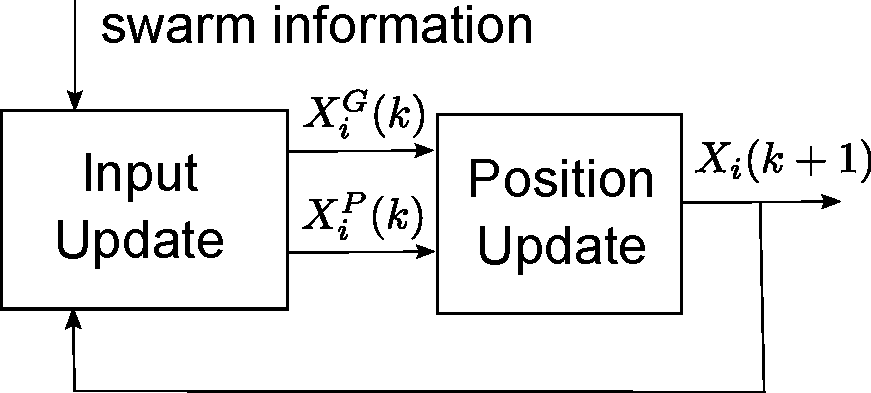
\includegraphics[width=0.6\linewidth]{sys_flow.pdf}
\caption{A system structure of the PSO}
\label{fig:sys_flow}
\end{figure}

We can decompose the model of a single particle into two components, which are illustrated in Figure \ref{fig:sys_flow}.
Two components forms a cascade system structure.
An \emph{optimization strategy sub-system} generates $ x^{G}_{i}(k) $ and $ x^{P}_{i}(k) $ based on last position $ x_{i}(k) $ and the swarm information from the topology interaction.
$ x^{G}_{i}(k) $ and $ x^{P}_{i}(k) $ are used as inputs to the \emph{rule update sub-system}.

The convergence problem are answered by
\begin{itemize}
\item whether the \emph{rule update sub-system} is input-to-state stable;
\item how the output of the \emph{optimization strategy sub-system} is like.
\end{itemize}

If the \emph{rule update sub-system} is input-to-state stable, the convergence of $ x_{i}(k) $ depends on the boundaries of $ x^{G}_{i}(k) $ and $ x^{P}_{i}(k) $.
In the next section, we will evaluate the input-to-state stability of the rule update sub-system.



\section{Input-to-State Stability of the Position Update}
\label{sec:iss}

In this section, we briefly review the definition of input-to-state stability (ISS) including both the conditions that guarantee it and the bound that ISS implies\cite{Jiang2001857}. 
We then show that PSO satisfies this definition when the parameters of PSO are set in the requisite range. We also derive the bounds implied by the ISS property.
We use the ISS property in Section \ref{sec:opt_strgy} to find bounds on particle motion.

We first introduce several types of functions \cite{Jiang2001857}.
\begin{itemize}
\item $ K $-function $ \mathbb{K} $ : a function $ \alpha  : [ 0, a ) \rightarrow [ 0, \infty ) $ is continuous, strictly increasing and $ \alpha (0) = 0 $; it is a $ K_{\infty} $-function, if $ \alpha (s) \rightarrow \infty $ as $ s \rightarrow \infty $;
\item $ KL $-function $ \mathbb{KL} $ : a function $ \beta : [ 0, a ) \times [ 0 , \infty ) \rightarrow [ 0, \infty ) $ satisfies:
\begin{enumerate}
\item $ \forall t \geq 0 $, $ \beta (\cdot , t ) $ is a $ K $-function;
\item $ \forall s \geq 0 $, $ \beta (s, \cdot) $ is decreasing and $ \beta(s,t) \rightarrow 0 $ as $ t \rightarrow \infty $.
\end{enumerate}
%\item Positive-definite function: a function $ \gamma (s) > 0, \forall s > 0 $ and $ \gamma (0) = 0 $.
\item ISS-Lyapunov function $ V : \mathbb{R}^{n} \rightarrow \mathbb{R}_{\geq 0} $ satisfies:
\begin{enumerate}
\item $ \exists \alpha_{1}, \alpha_{2} \in \mathbb{K} $ such that 
$ \forall \xi \in \mathbb{R}^{n}, \alpha_{1} ( | \xi | ) \leq V( \xi ) \leq \alpha_{2}  ( | \xi | ) $.
\item $ \exists \alpha_{3} \in \mathbb{K}_{\infty} , \sigma \in \mathbb{K} $ such that $ \forall \xi \in \mathbb{R}^{n}, \forall \mu \in \mathbb{R}^{m}, V( f( \xi, \mu ) ) - V( \xi ) \leq - \alpha_{3} ( | \xi | ) + \sigma ( | \mu | ) $. 
\end{enumerate}
\end{itemize}

\begin{mydef}[Input-to-state stable]\cite{Jiang2001857}
\label{def:iss}
For a discrete-time system
\begin{equation}
\label{eq:dis_nonlinear}
x(k+1) = f( x(k) , u(k) ),
\end{equation}
with $ f(0,0) = 0 $
\footnote{This means that $ x = 0 $ is an equilibrium of the 0-input system.}, the system is \emph{(globally) input-to-state stable} if there exist a $ KL $-function $ \beta  $ and a $ K $-function $ \gamma $ such that, for each input $ u \in l^{m}_{\infty} $ and each $ \xi \in \mathbb{R}^{n} $, it holds that $  \forall k \in \mathbb{Z}^{+} $,
\begin{equation}
\label{eq:def_iss}
| x(k, \xi, u) | \leq \beta (| \xi |, k) + \gamma (|| u ||).
\end{equation}
\end{mydef}

The $ \beta () $ term in equation \eqref{eq:def_iss} defines an initial bound with a decaying property.
The $ \gamma () $ term in equation \eqref{eq:def_iss} defines a bound determined by the input.
This means that the influence $ \beta () $ term gradually decreases to zero and the position is bounded by a range determined by the bound on the input.
An ISS-Lyapunov function, defined above, can be used to prove the input-to-state stability of a system and analyze the state bound\cite{Jiang2001857}.
We will use the ISS-Lyapunov-function approach in the proof given later in this section.

\subsection{Conditions for input-to-state stability for position update in PSO}

Using the definition of the PSO position update as given in equation \eqref{eq:pso_up_linalg_simp}, PSO can be shown to be ISS as defined in definition \ref{def:iss}.

\begin{mythm}
\label{thm:iss}
The system \eqref{eq:pso_up_linalg_simp} is input-to-state stable, when $ | \lambda_{\max} ( A(k) ) | < 1 $.
%The system \eqref{eq:pso_up_linalg_simp} is input-to-state stable, if there exists a symmetric positive definite matrix $ P $ and a symmetric positive definite matrix $ Q' $ that has $ A(k)^{T} P A(k) - P = - Q(k) \leq - Q' $.
\begin{proof}

Let $ P $ be an identity matrix.
As $ | \lambda_{\max} ( A(k) ) | < 1 $, we have
$ \lVert A^{T}(k) P A(k) \rVert \leq \lVert P \rVert \lVert A(k) \rVert^{2} \leq \lVert P \rVert | \lambda_{\max} ( A(k) ) |^{2} < \lVert P \rVert $.
Because $ P $ is an identity matrix it is positive definite, and thus $ A^{T}(k) P A(k) $ is positive definite or positive semi-definite by definition.
So by positive definite ordering we have $ A^{T}(k) P A(k) < P $.

Let $ -Q(k) = A^{T}(k) P A(k) - P $. Since $ A^{T}(k) P A(k) < P $ then $ - Q(k) < 0 $ furthermore $ \exists Q' \forall k, Q(k) > Q' > 0 $. 

By the Lemma 3.5 in \cite{Jiang2001857}, if we can show that a proposed positive definite Lyapunov function is an ISS-Lyapunov function, then the system is ISS.

Define a Lyapunov function
\begin{equation}
\label{eq:lyapunov_v}
V( X(k) ) = X^{T} (k) P X(k).
\end{equation}
We can have
$
\lambda_{min}(P) | X(k) |^{2} \leq V( X(k) )\leq \lambda_{max}(P) | X(k) |^{2}
$ and $ \lambda_{min}(P) = \lambda_{max}(P) $.

Let $ \alpha_{1} ( \xi )= \lambda_{min} \xi^{2} $
and 
$ \alpha_{2} ( \xi )= \lambda_{max} \xi^{2} $,
we have $ V(x) $ satisfying condition 1 of the ISS-Lyapunov function definition.

By applying equation \eqref{eq:pso_up_linalg_simp} to $ V( X(k+1) ) - V( X(k) ) $, we have
\begin{equation}
\label{eq:lyapunov_delta2}
\begin{aligned}
& V( X(k+1) ) - V( X(k) ) \\
= & - X^{T}(k) [ A^{T}(k) P A(k) - P ] X(k) \\
& + 2 X^{T}(k)  A^{T}(k) P B(k) U(k) + U^{T}(k) B^{T}(k) P B(k) U(k) \\
\leq & - X^{T}(k) Q' X(k) + 2 X^{T}(k)  A^{T}(k) P B(k) U(k) \\
& + U^{T}(k) B^{T}(k) P B(k) U(k) \\
\leq & - \lambda_{min}(Q') | X(k) |^{2} + 2  \lVert A^{T}(k) P B(k) \rVert | U(k) | | X(k) | \\
& + \lVert B^{T}(k) P B(k) \rVert | U(k) |^{2}.
\end{aligned}
\end{equation}

By completing the square, we have
\begin{equation}
\label{eq:lyapunov_delta4}
\begin{aligned}
& V( X(k+1) ) - V( X(k) ) \\
\leq & - \frac{1}{2} \lambda_{min}(Q') | X(k) |^{2} \\
& + \left[ \frac{2 \lVert A^{T}(k) P B(k) \rVert^{2}}{ ( \lambda_{min}(Q') )^{2} } + \lVert B^{T}(k) P B(k) \rVert \right] | U(k) |^{2}. 
\end{aligned}
\end{equation}

Because $ u^{P}(k) \in [0, 1] $, there exist an $ A' $ and $ B' $ such that $ \lVert A(k) \rVert \leq \lVert A' \rVert $ and $ \lVert B(k) \rVert \leq \lVert B' \rVert $.
We have $ \lVert A^{T}(k) P B(k) \rVert \leq \lVert A' \rVert \lVert P \rVert \lVert B' \rVert $ and $ \lVert B^{T}(k) P B(k) \rVert \leq \lVert P \rVert \lVert B' \rVert^{2} $.

Since the identity matrix $ P $ has $ || P || = 1 $:
\begin{equation}
\label{eq:lyapunov_delta5}
\begin{aligned}
& V( X(k+1) ) - V( X(k) ) \\
\leq & - \frac{1}{2} \lambda_{min}(Q') | X(k) |^{2} + [ \frac{2 \lVert A' \rVert^{2} \lVert B' \rVert^{2}}{ ( \lambda_{min}(Q') )^{2} } + \lVert B' \rVert^{2} ] | U(k) |^{2}.
\end{aligned}
\end{equation}

Let
$ \alpha_{3} ( \xi )= \frac{1}{2} \lambda_{min}(Q') \xi^{2} $,
and
$ \sigma ( \xi ) = [ \frac{2 \lVert A' \rVert^{2} \lVert B' \rVert^{2}}{ ( \lambda_{min}(Q') )^{2} } +  \lVert B' \rVert^{2} ] \xi^{2} $.
Thus we have $  V( X(k+1) ) - V( X(k) ) $ satisfying condition 2 of the ISS-Lyapunov function definition and
so \eqref{eq:lyapunov_v} is an ISS-Lyapunov function.
Using Lemma 3.5 in \cite{Jiang2001857}, the position update component of PSO (equation \eqref{eq:pso_up_linalg_simp}) is input-to-state stable.

\end{proof}
\end{mythm}

Note that in using equation \eqref{eq:pso_up_linalg_simp},
$ [ v(k), x(k) - x^{*} ]^{T} = [0, 0]^{T} $ is an equilibrium position when the input $ [ x^{G}(k) - x^{*} , x^{P}(k) - x^{*} ]^{T} = [0, 0]^{T} $.
For an arbitrary optimization problem $ x^{*} $ would typically not be at the origin. 
In such a problem, input-to-state stability means that the boundaries of $ | v(k) | $ and $ | x(k) - x^{*} | $ would be transformed and thus determined by $ | x^{G}(k) - x^{*} | $ and $ | x^{P}(k) - x^{*} | $,
but the properties of ISS still apply independent of where the function is centered.

Having proven that PSO is ISS we can now state a bound on particle position.

\begin{mycoro}
\label{coro:state_bound}
Given the bound on the input $ || u || $ in the position update component, we have the bound on the particle position from equation \eqref{eq:pso_up_linalg_simp}.
\begin{equation}
\label{eq:state_bound}
\forall k, 
| x(k) - x^{*} | \leq \max ( | x(0) - x^{*} | , \gamma ( | [ x^{G}(k) - x^{*}, x^{P}(k) - x^{*} ]^{T} | ) ),
\end{equation}
in which $ \gamma = \alpha_{3}^{-1} \circ \sigma $.

The $ \max $ part is needed to account for the effect of the starting point, represented by the first parameter. Eventually the effect of the starting point no longer affects the system, formally:
\begin{equation}
\label{eq:state_bound:conv}
\exists T, \forall k \geq T, 
|  x(k) - x^{*} | \leq \gamma ( | [ x^{G}(k) - x^{*}, x^{P}(k) - x^{*} ]^{T} | ).
\end{equation}
\begin{proof}
This is obtained from Remark 3.7 in \cite{Jiang2001857} and by choosing $ P $ be a symmetric identity matrix.
Furthermore we drop the velocity part becuase $ | x(k) - x^{*} | \leq | [ v(k), x(k) - x^{*} ]^{T} | $.
\end{proof}
\end{mycoro}

Figure \ref{fig:boundary} gives an example on how a particle's boundary is determined by the personal best and global best.

\begin{figure}
\centering
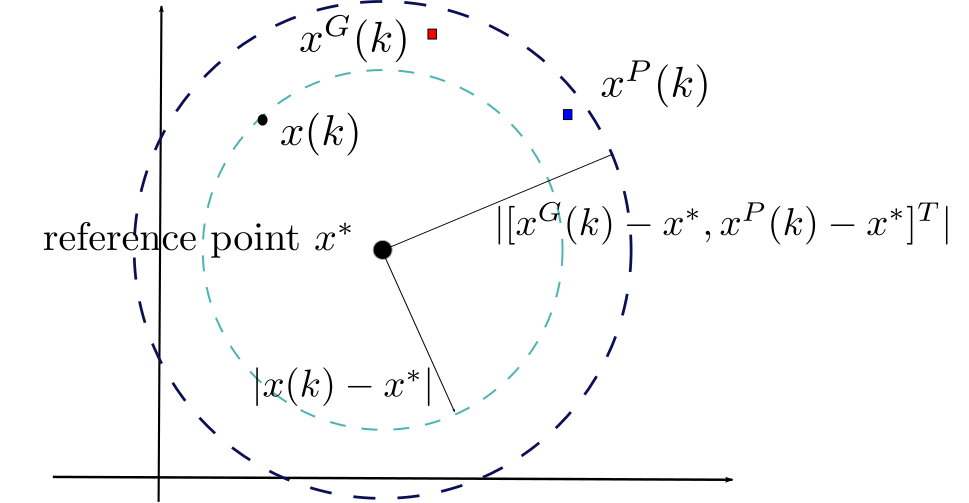
\includegraphics[width=0.9\linewidth]{./figure/boundary}
\caption{A bound on a particle's position by a reference point $ x^{*} $ from Equation \ref{eq:state_bound:conv}.
The ratio of wo radii indicates $ \gamma $.}
\label{fig:boundary}
\end{figure}

\begin{mycoro}
\label{coro:param_unit_disc}
Write $ A(k) = 
\begin{bmatrix}
\chi & - \chi \phi \\
\chi & 1 - \chi \phi
\end{bmatrix}
$, in which
$ \phi \in [0,  \phi^{P} + \phi^{G} ] $ and $ \chi \in ( 0, 1 ) $.
When $ \phi \in (0 , \frac{2(1+\chi)}{\chi} ) $, the system \eqref{eq:pso_up_linalg_simp} is input-to-state stable.
\begin{proof}
Let $ a = (1 + \chi) - \chi \phi $. 
The eigenvalues of $ A(k) $ are
$ \lambda = \frac{ a \pm \sqrt{ a^{2} - 4 \chi } }{2} $.

\begin{enumerate}
\item If $ a^{2} \geq 4 \chi $, we have $ a \geq 2 \sqrt{\chi} $ or $ a \leq - 2 \sqrt{\chi} $.

If $ a \geq 2 \sqrt{\chi} $, then $ | \lambda_{\max} | < 1 $ derives $ 0 < \frac{a-\sqrt{a^{2}-4\chi}}{2} \leq \frac{a+\sqrt{a^{2}-4\chi}}{2} < 1 $.
It means that $ 2 \sqrt{ \chi } \leq a < 1 + \chi $.

If $ a \leq 2 \sqrt{\chi} $, then $ | \lambda_{\max} | < 1 $ derives $ -1 < \frac{a-\sqrt{a^{2}-4\chi}}{2} \leq \frac{a+\sqrt{a^{2}-4\chi}}{2} < 0 $.
It means that $ - (\chi+1) < a \leq - 2 \sqrt{\chi} $.

\item If $ a^{2} \geq 4 \chi $, we have $ - 2 \sqrt{\chi} < a < 2 \sqrt{\chi} $.

$ | \lambda_{\max} | < 1 $ derives $ \frac{ a^{2} }{4} + \frac{ a^{2} - 4\chi }{4} < 1 $.
It means that $ - 2 \sqrt{ 2(1+\chi) } < a < 2 \sqrt{ 2(1+\chi) } $.
Because $ \sqrt{ 2(1+\chi) } > 2 \sqrt{ \chi } $, we have $ - 2 \sqrt{\chi} < a < 2 \sqrt{\chi} $.
\end{enumerate}
Combining these two cases, we have  $ - (1 + \chi) < a < 1 + \chi $.
It equals to $ \phi \in (0 , \frac{2(1+\chi)}{\chi} ) $.

\end{proof}
\end{mycoro}

Figure \ref{fig:paramSpace} shows the parameter space.
The x-axis is $ \phi = \phi^{P} + \phi^{G} $ and the y-axis is $ \chi $.
The stable region in red is obtained from eigenvalue test on Theorem \ref{thm:iss} and the yellow boundary is obtained from Corollary \ref{coro:param_unit_disc}.
\begin{figure}
\centering
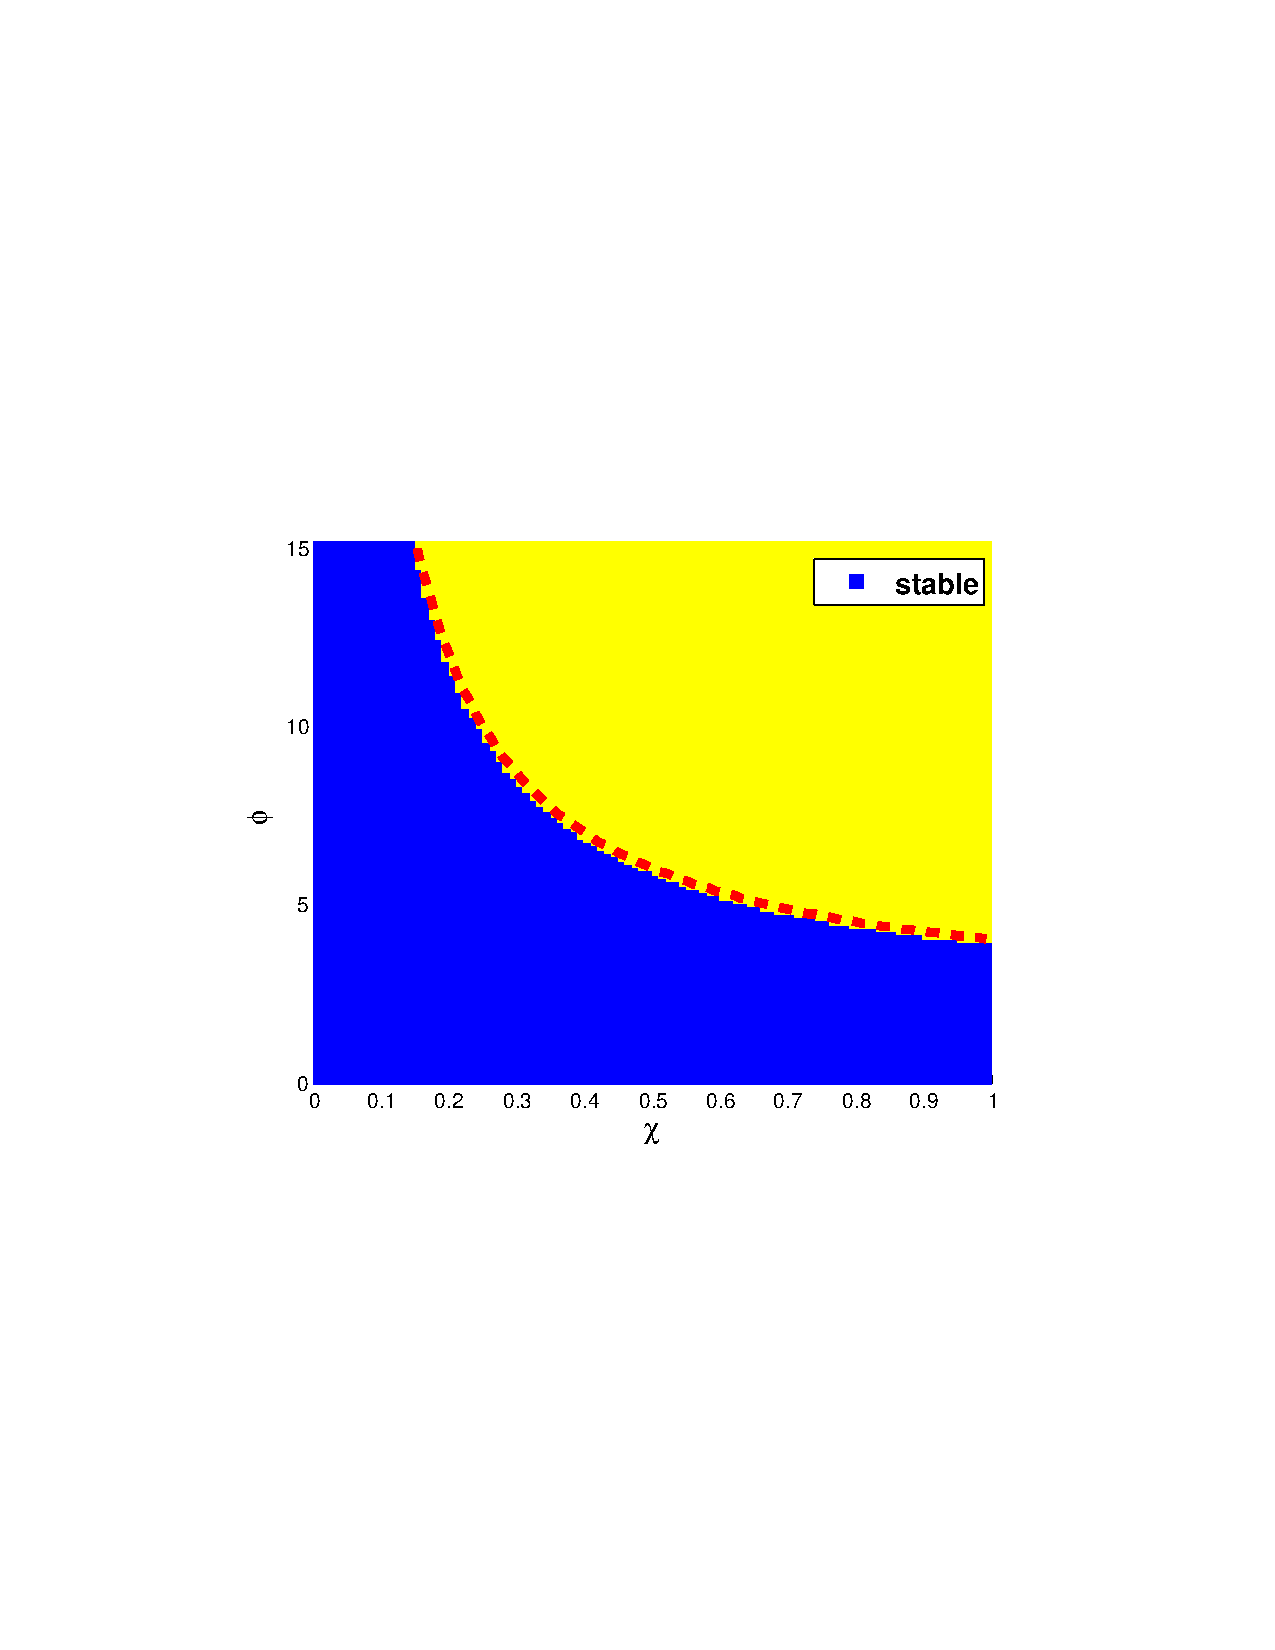
\includegraphics[width=0.9\linewidth]{./figure/param2}
\caption{Parameter space}
\label{fig:paramSpace}
\end{figure}

\begin{figure}
\centering
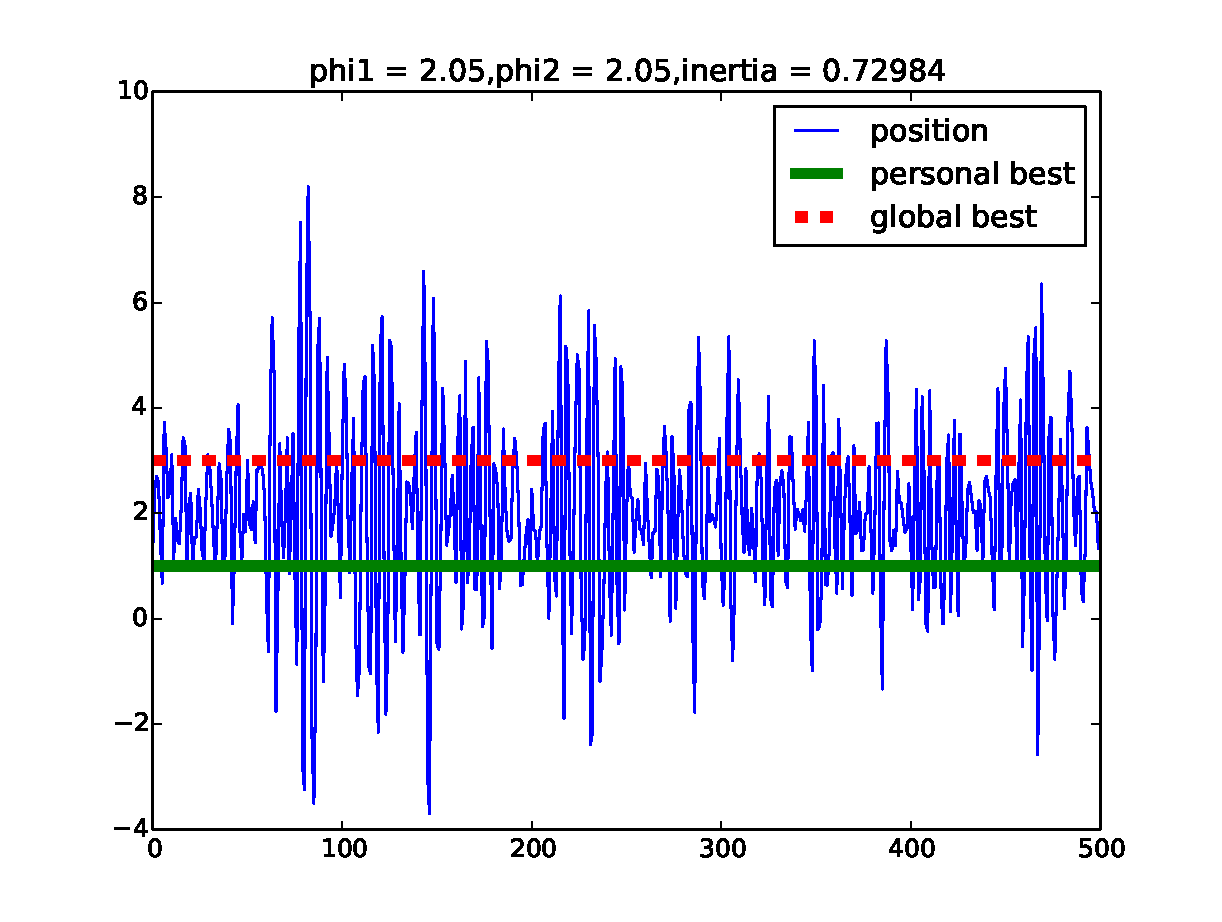
\includegraphics[width=\linewidth]{./figure/bound_case_1}
\caption{Parameters in the margin of stable region.}
\label{fig:bound_case:a}
\end{figure}

\begin{figure}
\centering
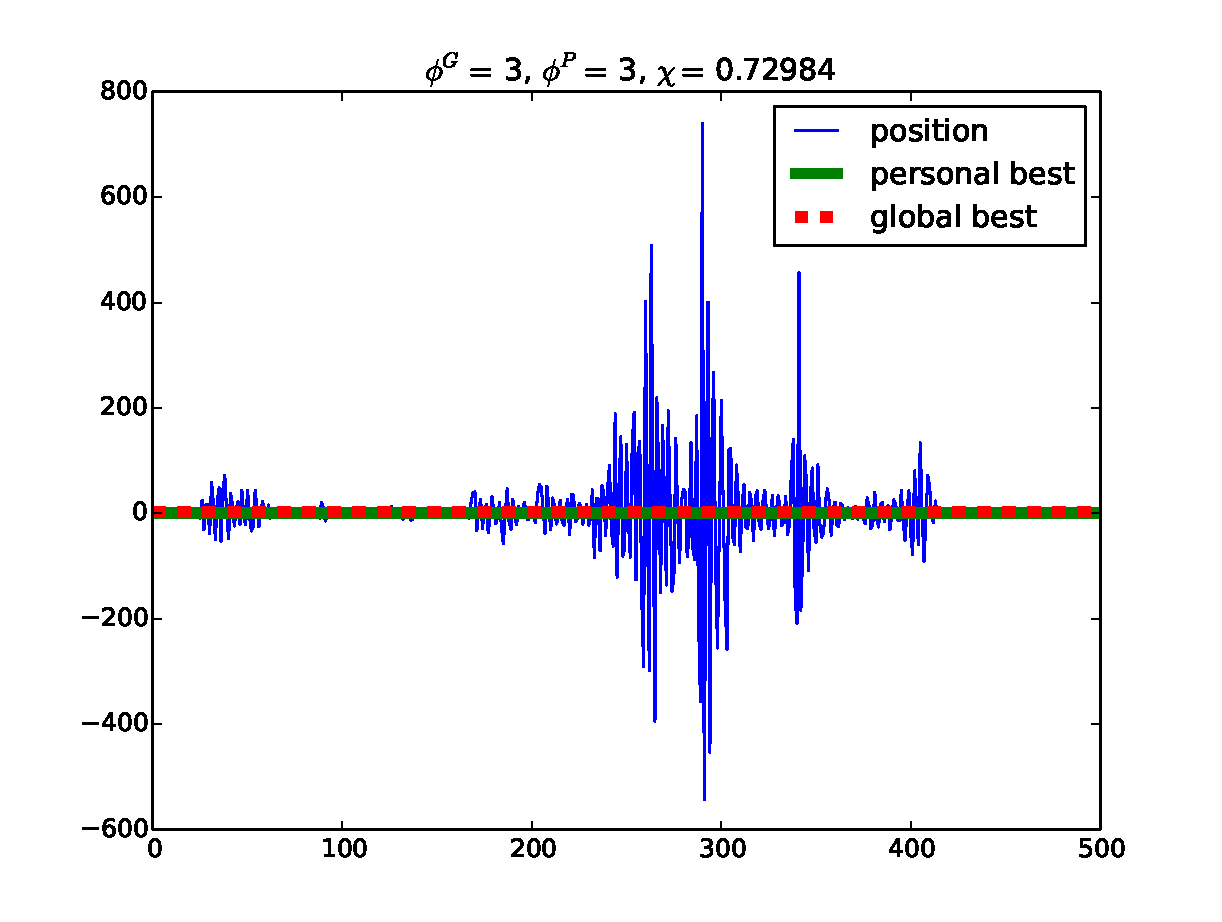
\includegraphics[width=\linewidth]{./figure/bound_case_2}
\caption{Parameters not in the stable region.}
\label{fig:bound_case:b}
\end{figure}

\begin{figure}
\centering
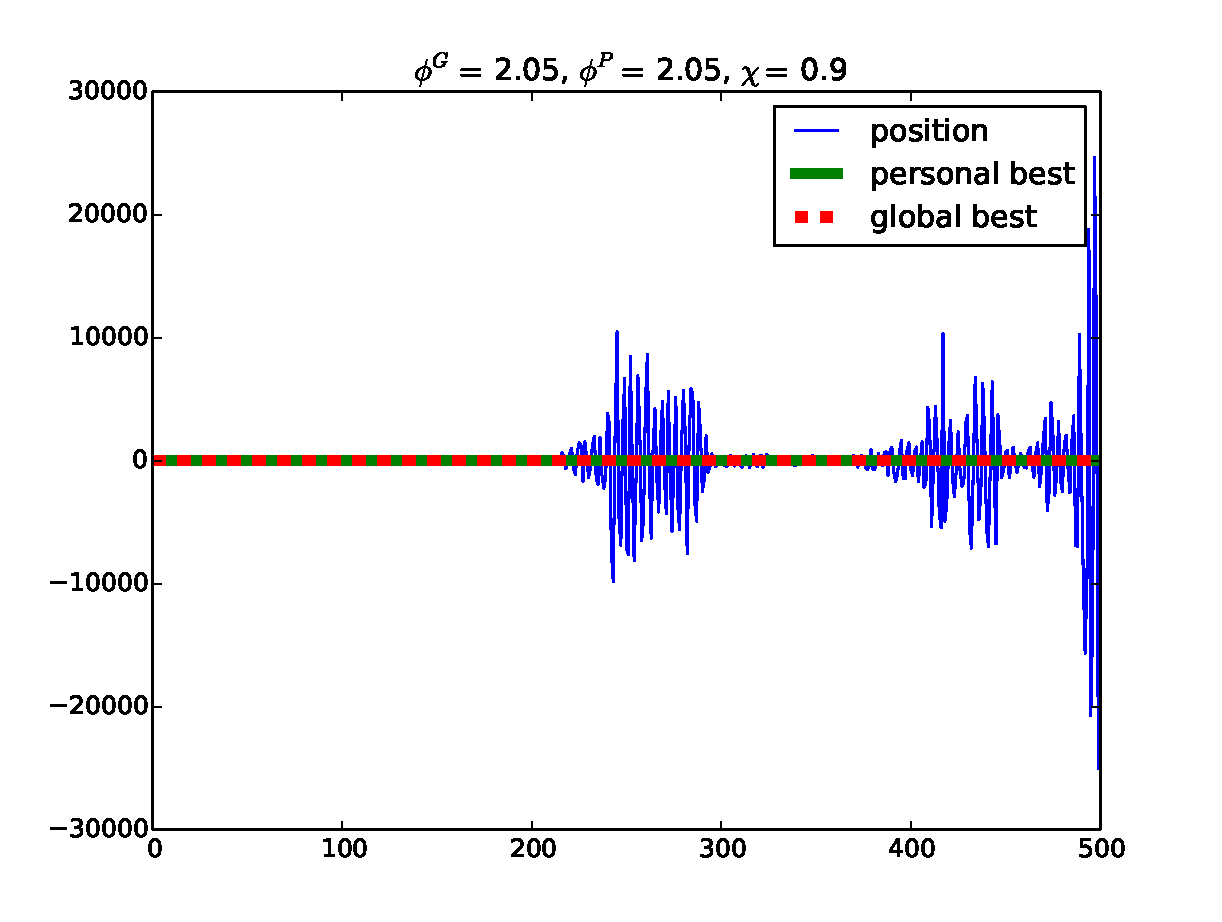
\includegraphics[width=\linewidth]{./figure/bound_case_3}
\caption{Parameters not in the stable region.}
\label{fig:bound_case:c}
\end{figure}

\begin{figure}
\centering
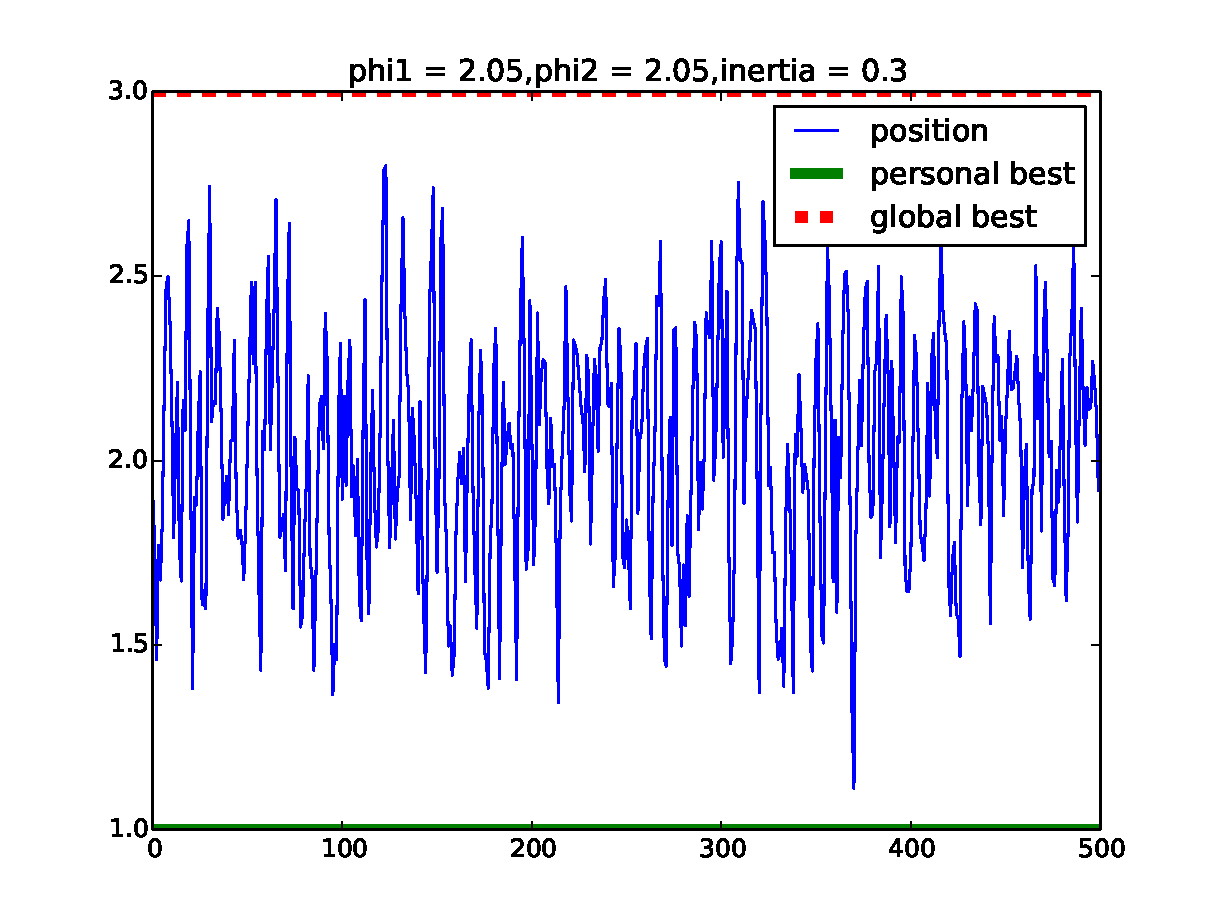
\includegraphics[width=\linewidth]{./figure/bound_case_4}
\caption{Parameters in the stable region.}
\label{fig:bound_case:d}
\end{figure}

\begin{figure}
\centering
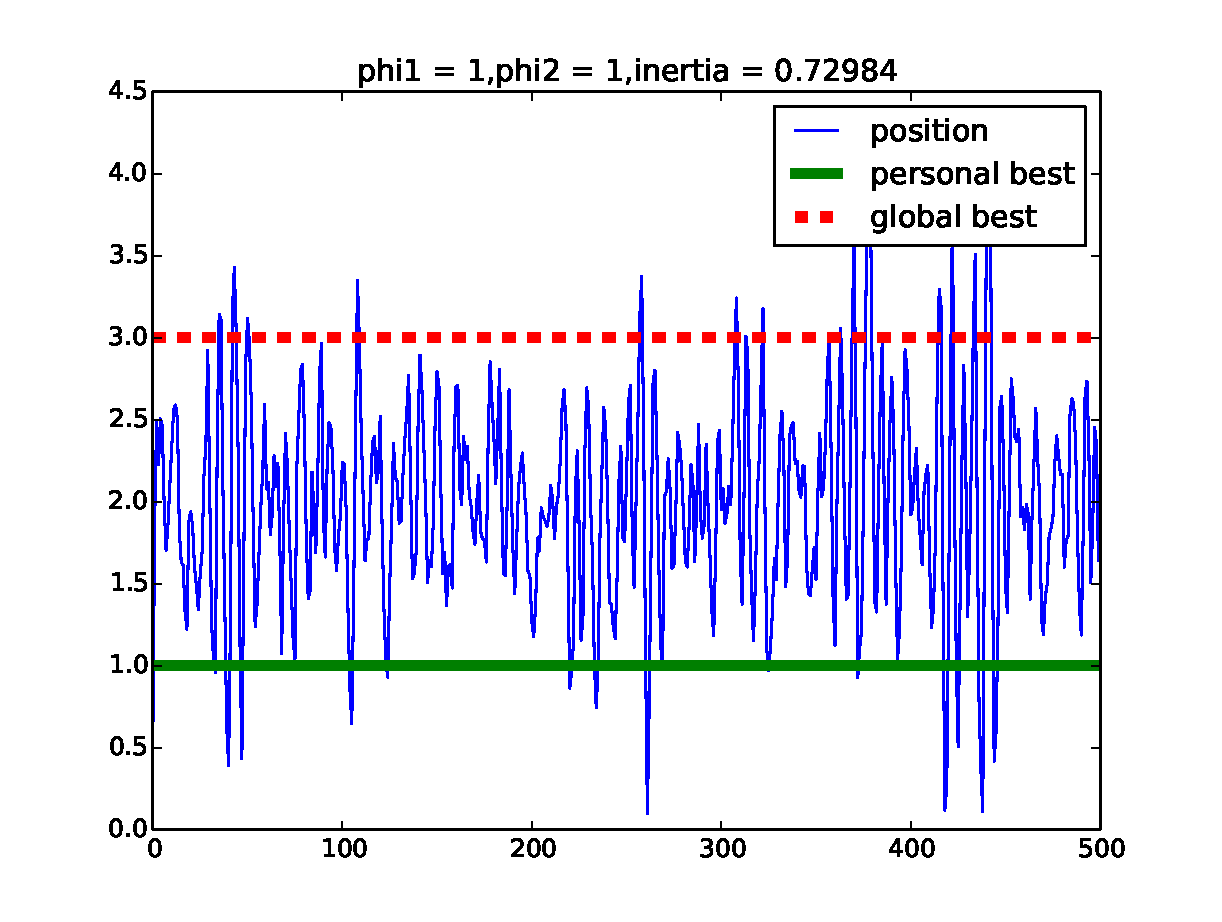
\includegraphics[width=\linewidth]{./figure/bound_case_5}
\caption{Parameters in the stable region.}
\label{fig:bound_case:e}
\end{figure}




\section{Optimization strategy}

When the rule update sub-system is input-to-state stable, the convergence of $ x(k) $ depends on the input $ u(k) $, which are $ x^{P}(k) $ and $ x^{G}(k) $ from the optimization strategy sub-system.
In the PSO algorithm, we are interested with how the particles converge to an interested position or area, where the optimal point locates.
The input-to-state stable is for the convergence to the origin.
By coordinator transformation, we can show that given a reference point, if the input is bounded in an area around the reference point, the output can also be bounded around the reference point.


\subsection{Single-objective optimization}

As the stagnation is defined as there is no new improvement found, we have that $ x^{P}(k) $ and $ x^{G}(k) $ are constant.
In \cite{985692}, it is stated that
\begin{equation}
\label{eq:single_obj_equilibrium}
\hat{x} = \frac{\phi^{P} x^{P} + \phi^{G} x^{G} }{ \phi^{P} + \phi^{G} } 
\end{equation}
 is an equilibrium point, in which $ x^{P} $ and $ x^{G} $ are the personal best and global best in stagnation respectively.

Let $ \hat{x} $ be the reference point and $ x^{*} $ be the optimal point, we know that 
\begin{equation}
\label{eq:single_obj_input_bound}
| U(k) | \leq \max (| x^{P} - \hat{x} |, | x^{G} - \hat{x} |).
\end{equation}



Particularly, when $ x^{P} = x^{*} $ and $ x^{G} = x^{*} $, we have
$ \hat{x} = x^{*} $.
Then $ | U(k) | = 0 $.
By definition \eqref{def:iss}, we know that
\begin{equation}
\label{eq:single_obj_convergence}
\exists T , | x(T) - x^{*} |  = 0,
\end{equation}
which means that $ x(k) \rightarrow x^{*} $. 

\subsection{Multi-objective optimization}
\cite{Chakraborty20111411} looks at the convergence in the multi-objective optimization problem.

In this case, 


\section{Stochastic Analysis}

The input-to-stable stability analysis can also be applied to stochastic analysis, like those in \cite{Jiang20078} and \cite{Poli:2008:DSS:1384929.1384944}.

\subsection{Mean convergence analysis}

In analyzing the mean of the dynamic, we are less interested with the mean of the velocity. 
We adopt a same way like \cite{Jiang2001857} to construct the mean\footnote{How it is derived is given in appendix \ref{sec:app:derivation_mean} }.

\begin{equation}
\label{eq:pso1_alg_mean_linalg:final}
\begin{bmatrix}
E( x(k+1) ) \\
E( x(k) )
\end{bmatrix}
=
\begin{bmatrix}
1 + \chi - a(k) - b(k) & -\chi \\
1 & 0
\end{bmatrix}
\begin{bmatrix}
E( x(k) ) \\
E( x(k-1) )
\end{bmatrix}
+
\begin{bmatrix}
a(k) & b(k) \\
0 & 0
\end{bmatrix}
\begin{bmatrix}
E( x^{P}(k) ) \\
E( x^{G}(k) )
\end{bmatrix}
\end{equation}

We are interested with how $ E( x(k) ) $ deviates from the optimal position $ x^{*} $.
Thus, we had a coordinator transformation to move from the origin $ [0, 0]^{T} $ to the origin $ [x^{*}, x^{*}]^{T} $.
Let
\begin{equation}
\label{eq:def_delta_ex}
\Delta E( x(k) ) = E( x(k) ) - x^{*},
\end{equation}
\begin{equation}
\label{eq:def_delta_exg}
\Delta E( x^{G}(k) ) = E( x^{G}(k) ) - x^{*}
\end{equation}
and
\begin{equation}
\label{eq:def_delta_exp}
\Delta E( x^{P}(k) ) = E( x^{P}(k) ) - x^{*}
\end{equation}

\begin{equation}
\label{eq:pso1_alg_mean_linalg:final:trans}
\begin{bmatrix}
\Delta E( x(k+1) ) \\
\Delta E( x(k) )
\end{bmatrix}
=
\begin{bmatrix}
1 + \chi - \frac{ \chi \phi^{P} }{2} - \frac{ \chi \phi^{G} }{2} & -\chi \\
1 & 0
\end{bmatrix}
\begin{bmatrix}
\Delta E( x(k) ) \\
\Delta E( x(k-1) )
\end{bmatrix}
+
\begin{bmatrix}
\frac{ \chi \phi^{P} }{2} & \frac{ \chi \phi^{G} }{2} \\
0 & 0
\end{bmatrix}
\begin{bmatrix}
\Delta E( x^{P}(k) ) \\
\Delta E( x^{G}(k) )
\end{bmatrix}
\end{equation}

The input-to-state stable analysis on equation \eqref{eq:pso1_alg_mean_linalg:final:trans} shows how the $ E(x(k)) $ will deviate from the $ x^{*} $ when we know how $ E( x^{G}(k) ) $ and $ E( x^{P}(k) ) $ deviate from the $ x^{*} $.
\begin{mythm}
The system \eqref{eq:pso1_alg_mean_linalg:final:trans} is input-to-state stable, if there exist a symmetric positive definite matrix $ P $ and a symmetric positive definite matrix $ Q $ so that
$ A^{T} P A - P = Q $ and
\begin{equation}
A =
\begin{bmatrix}
1 + \chi - \frac{ \chi \phi^{P} }{2} - \frac{ \chi \phi^{G} }{2} & -\chi \\
1 & 0
\end{bmatrix}.
\end{equation}
\end{mythm}


\subsection{Variance convergence analysis}

In analyzing the variance, we are interested with how the $ VAR(x(k)) $ deviates the origin.
There is no need to have a coordinator transformation.

The variance convergence analysis is usually based on that the mean has converged \cite{Jiang20078} \cite{Poli:2007:EAS:1276958.1276977}.
We have the means of $ x(k) $, $ x^{G}(k) $ and $ x^{P}(k) $ as constant, which are $ E(x(k)) = E(x) $, $  E(x^{G}(k)) = \bar{x}^{G} $. and $ E(x^{P}(k)) = \bar{x}^{P} $. 
For convenience, we have
\begin{equation}
\label{eq:def_delta_mean_xg}
E(x^{G}(k)) - E(x(k)) =  \bar{x}^{G} - E(x) = \Delta \bar{x}^{G}
\end{equation}
and
\begin{equation}
\label{eq:def_delta_mean_xp}
E(x^{P}(k)) - E(x(k)) =  \bar{x}^{P} - E(x) = \Delta \bar{x}^{P}.
\end{equation}

We have the variance model as\footnote{How it is derived is given in appendix \ref{sec:app:derivation_variance} }
\begin{equation}
\label{eq:pso1_alg_var_linalg}
\begin{aligned}
\begin{bmatrix}
VAR( x(k) ) \\
VAR( x(k-1) ) \\
VAR( x(k-2) ) 
\end{bmatrix}
= &
\begin{bmatrix}
- \chi + \alpha_{2}  &  \chi^{2} + \chi \alpha_{2} + 2 \chi ( \alpha_{1} )^{2}  & \chi^{2} \\
1 & 0 & 0 \\
0 & 1 & 0
\end{bmatrix}
\begin{bmatrix}
VAR( x(k-1) ) \\
VAR( x(k-2) ) \\
VAR( x(k-3) ) 
\end{bmatrix}
\\ & +
\begin{bmatrix}
\beta_{1} & \beta_{2} & \beta_{3} \\
0 & 0 & 0 \\
0 & 0 & 0
\end{bmatrix}
\begin{bmatrix}
VAR( x^{G}(k-1) ) \\
VAR( x^{P}(k-1) ) \\
1
\end{bmatrix},
\end{aligned}
\end{equation}
in which
\begin{equation}
\label{eq:def_param_alpha1}
\alpha_{1} = 1 + \chi - \frac{ \chi \phi^{G} }{2} - \frac{ \chi \phi^{P} }{2}
\end{equation}
\begin{equation}
\label{eq:def_param_alpha2}
\alpha_{2} = (1 + \chi - \chi \frac{ \phi^{G} + \phi^{P} }{ 2 } )^{2} - \frac{1}{6} \chi^{2} ( ( \phi^{G} )^{2} + ( \phi^{P} )^{2} ),
\end{equation}
\begin{equation}
\label{eq:def_param_beta1}
\beta_{1} = \frac{1}{12} \chi^{2} ( \phi^{G} )^{2},
\end{equation}
\begin{equation}
\label{eq:def_param_beta2}
\beta_{2} = \frac{1}{12} \chi^{2} ( \phi^{P} )^{2},
\end{equation}
and
\begin{equation}
\label{eq:def_param_beta3}
\beta_{3} = \frac{ \chi^{2} }{ 12 } [ (\phi^{G})^{2} (\Delta \bar{x}^{G} )^{2} + (\phi^{P})^{2} (\Delta \bar{x}^{P} )^{2} + 6 \phi^{G} \phi^{P} \Delta \bar{x}^{G} \Delta \bar{x}^{P} ].
\end{equation}

\begin{mythm}
The system \eqref{eq:pso1_alg_var_linalg} is input-to-state stable, if there exist a symmetric positive definite matrix $ P $ and a symmetric positive definite matrix $ Q $ so that
$ A^{T} P A - P = Q $ and
\begin{equation}
A = 
\begin{bmatrix}
- \chi + \alpha_{2}  &  \chi^{2} + \chi \alpha_{2} + 2 \chi ( \alpha_{1} )^{2}  & \chi^{2} \\
1 & 0 & 0 \\
0 & 1 & 0
\end{bmatrix}.
\end{equation}
\end{mythm}

\section{Conclusion}
\label{sec:conclusion}

In this paper, we have decomposed the PSO algorithm into a cascade model, which consists of input update and position update components.
We introduce the input-to-state stability analysis to the position update component.
For an input-to-state stable position update component, if the input to this component is bounded, the state is bounded; also if the input to the component converges, the state converges.
The convergence of the PSO is determined by the output of the input update component, which are the personal best and global best.
If they are in stagnation, the particle converges.

The analysis of a cascade structure used here can be applied to a wide range of the PSO variants.
In cases that use the same position update component but different input update components, the convergence and the boundary of the particles are determined by
whether the input update component generates converging or bounded personal best and global best.
For variants that use a different position update component, the ISS properties would need to be verified.


\bibliographystyle{IEEEtran}
\bibliography{reference}


\end{document}

